\section{Kalman Filters}

The concept of the Kalman filter was first published by Rudolph E. Kalman in 1960 in his paper ``A new approach to linear filter and prediction problems''. Kalman sought to create a new method of estimating linear dynamic systems that was more practical to use with machine computation. Kalman explains, ``Present methods for solving the Wiener problem (linear dynamic systems) are subject to a number of limitations which seriously curtail their practical usefulness.'' [1] Kalman details his newly invented algorithm which provides efficient computational means to recursively estimate the state and error covariance of a process, in a way that minimizes the mean of the squared error covariance [2]. The algorithm, now dubbed the Kalman filter, is a set of mathematical equations broken up into two steps: Prediction and Update described in detail below.

Today the Kalman filter is used in several modern applications such as sensor fusion/filtering, data smoothing, and forecasting/prediction [1] [3] [4] [5]. The traditional Kalman Filter (KF) is a tool used to analyze a set of linear data points for an unknown dynamic model. Each data point is passed in 1-by-1 to the filter (thus the k$^{th}$ step involves the k$^{th}$ data point) using the following nomenclature:\newline

$\bm{\hat{x}_{k|k}}$ [$\mathbb{R}^{n}$]:    the k$^{th}$ estimated state space given the first k observations ($z_{1} \cdots z_{k}$)\newline
$\bm{\hat{x}_{k|k-1}}$ [$\mathbb{R}^{n}$]:  the k$^{th}$ estimated state space given the first k-1 observations ($z_{1} \cdots z_{k-1}$)\newline
$F_{k}$ [$\mathbb{R}^{n\times n}$]:  the state transition function\newline
$B_{k}$:   the control input model \newline
$U_{k}$:   the input conrol vector\newline
$P_{k|k}$ [$\mathbb{R}^{n\times n}$]:  the error covariance matrix of (the confidence in) $x_{k|k}$\newline
Q [$\mathbb{R}^{n\times n}$]:    the processing noise (confidence in the predictions)\newline
$H_{k}$ [$\mathbb{R}^{1\times n}$]: the observation model at step k\newline
$z_{k}$ [$\mathbb{R}$]: the k$^{th}$ observation\newline
$y_{k}$ [$\mathbb{R}$]: the k$^{th}$ estimate residual\newline
R [$\mathbb{R}$]: the measurement noise (confidence in the obervations)\newline
$S_{k}$ [$\mathbb{R}$]: the innovation covariance\newline
$K_{k}$ [$\mathbb{R}^{n\times}$]: the kalman gain\newline

Assuming a state space with $n$ parameters, each of these is a matrix of dimension [${\rm I\!R}^{dxe}$] meaning it has $d$ rows and $e$ columns. For each dataset there exists a proper pairing of $Q$ and $R$ , however, they are usually not known. They represent artifacts of the Kalman filters' assumptions that the noise in the data is Gaussian (normally distributed) with mean 0 (i.e. white noise). $Q$ is the covariance matrix of a multivariate normal distribution centered at $\bm{\mu}$

\begin{equation}
    \bm{\mu} = [\mu_{1}, \cdots , \mu_{n}], \quad \mu_{i} = 0
\end{equation}

 where $n$ is the number of elements in the state space $\hat{x}_{k}$. $Q$ then represents the assumed known variability in each of the n parameters in $\bm{\hat{x}_{k}}$. Larger entries in $Q$ corresponds to larger variability in x which implies a lower confidence in the predicted $\hat{x}_{k}$. $R$ is the variance of a univariate normal distribution centered at 0. This acts as the assumed known variability in all observations $z_{k}$.

Given the appropriate values of $Q$ and $R$, the KF acts as an optimal estimator as it minimizes the Mean Square Error (MSE) of the predicted $\bm{\hat{x}}$. In practice, this can be thought of as nearly equivalent to a recursive weighted least squares (WLS) estimate where $Q$ acts as the forgetting factor for the KF similar to how $W$ does in WLS. It should be noted this only works for our application because we provide the data in chronological order. In practice, the Kalman Filter can predict on data provided in any order so $Q$ will more quickly "forget" the earlier data points provided. However, determining a proper $Q-R$ pair for a set of data can often be very difficult as it is still an open problem.

\subsection{Parameter Estimation with Kalman Filters}
Normally, the Kalman Filter is used to smooth out noise while maintaining the general form of the original data. As seen in Figure \ref{fig:kfexamp}, the KF can take a set of noisy observations and is able to reconstruct a good approximation of the true function's behavior. However, with minor adjustments to the algorithm, it can be converted from predicting function values to predicting function parameters.

\begin{figure}[h]
\centering
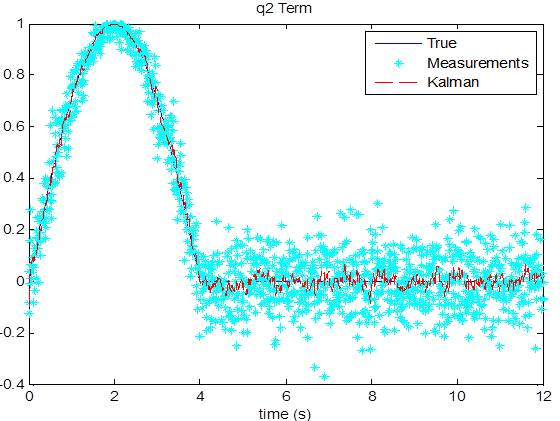
\includegraphics{body/methodology/q2_kalman.jpg}
\caption[Kalman Filter Graphic Example]{Example showing how the Kalman Filter is capable of taking in a set of noisy data (blue) and derives a smoothed estimate (red) that is generally accurate to the true function (black).}
\label{fig:kfexamp}
\end{figure}

%  For our application, we chose to instead use it to approximate the parameters to a function that best fits the data and from those parameters, then forecast what the value should be at some time in the future. Our implementation is as follows:

We will assume we have a set of noisy linear data of the form (time, value) such that we want to find the best linear approximation of the form 

\begin{equation} 
V = \hat{\alpha} + \hat{\beta}T
\end{equation}

that fits this data. We start with an initial state space estimate of $\bm{\hat{x}_{0|0}}$, error covariance matrix estimate $P_{0|0}$ and chosen values of $Q$ and $R$.

\begin{subequations}
\begin{align}
    \bm{x_{0|0}} &= \begin{bmatrix}
           \alpha \\
           \beta
         \end{bmatrix}
 \end{align}
  \begin{align}
    P_{k} &= \begin{bmatrix}
           P_{\alpha}&0 \\
           0&P_{\beta}
         \end{bmatrix}
  \end{align}
  \begin{align}
    Q &= \begin{bmatrix}
        Q_{\alpha}&0 \\
        0&Q_{\beta}
        \end{bmatrix}
  \end{align}
  \end{subequations}
  
  \subsubsection{KF Prediction}
  
  The first step is prediction. We calculate $\bm{x_{k|k-1}}$ and $P_{k|k-1}$ at the current iteration based on the last iteration's predicted $\bm{x_{k-1|k-1}}$ and $P_{k-1|k-1}$.
  
  \begin{subequations}
  \begin{align}
  \bm{\hat{x}_{k|k-1}} = F_{k} \bm{\hat{x}_{k-1|k-1}}+B_{k}u_{k}   \\
  P_{k|k-1} = F_{k} P_{k-1|k-1}F_{k}^{T}+Q
  \end{align}
  \end{subequations}
  
  For our purposes, assume $F_{k}$ is always identity, meaning the model does not change with time. We also assume $B_{k}u_{k} = 0$.
  
  \begin{align}
    F_{k} &= \begin{bmatrix}
           1&0 \\
           0&1
         \end{bmatrix}
  \end{align}
  
  Since any matrix multiplied by identity is always the original matrix, this reduces Equations 2.17a and 2.17b to the form
  
  \begin{subequations}
  \begin{align}
  \bm{\hat{x}_{k+1|k}} = \bm{\hat{x}_{k|k}}  \\
  P_{k+1|k} = P_{k|k}+Q
  \end{align}
  \end{subequations}
  
  This is a simplification in our application, as we know the true function is not constant as can be seen from figures 2.4 - 2.6. These changes shift the filter from a dynamic to a nearly static model approximation. $P$ represents the confidence in (or variability of) each parameter in the current state space with larger values of $P$ implying less confidence in $\bm{\hat{x}}$. From equation 2.19b, we can see that providing a larger $Q$ causes consistently larger estimates of $P$. This makes sense as $Q$ is a measure of the variability in each parameter of $\bm{\hat{x}}$, so larger $Q$'s should cause the KF to be less confident in it's predictions.
  
  As a further simplification, assumed $P$ and $Q$ to be 0 in the off diagonal as in equations 2.16b and 2.16c. This assumes that the parameters $\alpha$ and $\beta$ exist and change independent of eachother where  P$_{\alpha}$,  P$_{\beta}$, Q$_{\alpha}$, and Q$_{\beta}$ can be any non-negative real numbers.
 
 \subsubsection{KF Updating}
 
  The second step is updating. Each iteration of the KF utilizes a single data point, so the k$^{th}$ iteration will use the point ($t_{k}$, $v_{k}$). We begin by calculating the residual (or error from the k$^{th}$ known observation) for ($t_{k}$, $v_{k}$).
  
  \begin{equation}
  \centering
  y_{k} = z_{k} - H_{k}\bm{\hat{x}_{k|k-1}}
  \end{equation}
  
  Here H$_{k}$ is
  
  \begin{align}
    H_{k} &= \begin{bmatrix}
           1&t_{k}
         \end{bmatrix}
  \end{align}
  
  From equation 2.16a, we can see 
  
  \begin{equation}
  \centering
    H_{k}\bm{\hat{x}_{k|k-1}} = \alpha + \beta t_{k} = \hat{v}_{k}
  \end{equation}
  
  Thus, y$_{k}$ is simply the difference between the prediction of $\hat{v}_{k}$ at $t_{k}$ and the actual observed $v_{k}$ at $t_{k}$.
  
  We then perform the innovation step to calculate $s_{k}$. $s_{k}$ can be understood as a metric for the confidence in observation $z_{k}$ as it represents the variability of the first $k$ observations ($z_{1}, \cdots , z_{k}$). If the values of $z_{1 \cdots k}$ tend to vary greatly, $s_{k}$ will be large. If the values of $z_{1 \cdots k}$ only vary slightly, $s_{k}$ will be small. Larger values of $R$ also cause larger values of $s_{k}$ as seen in equation 2.23 since $R$ is a measure of the variability for all observations.
  
  \begin{equation}
  \centering
    s_{k} = R + H_{k}P_{k|k-1}H_{k}^{T}
  \end{equation}
  
  $P$, $H$, and $s$ come together to form $K_{k}$, the Kalman gain. Kalman gain can be thought of as a ``velocity factor'' of sorts for the KF controlling the magnitude of adjustment to make to the current $\bm{\hat{x}_{k}}$. The formula for the optimal gain, meaning it minimizes the mean square error of the estimate, is  
  
    \begin{equation}
  \centering
    K_{k} = P_{k|k-1}H_{k}^{T}s_{k}^{-1}
  \end{equation}
  
  From this we can see that as $P_{k}$ gets small, so too does $K_{k}$. This is because a small $P_{k}$ implies high confidence (or low variability) in $\bm{\hat{x}_{k}}$. Thus, having high confidence in the current state should yield only a small change to the new predicted $\bm{\hat{x}_{k}}$. We can also see that as $s_{k}$ gets large, $K_{k}$ gets small. This also makes sense since large $s_{k}$ implies low observation confidence (or high observation variability). In that case we'd want a smaller state adjustment for larger prediction errors as we don't trust the current observation as true (that is we want our state adjustment to be less sensitive to erroneous predictions).
  
  We then improve the current state space estimate using information from the $k^{th}$ iteration thus transitioning from $\bm{\hat{x}_{k|k-1}}$ to $\bm{\hat{x}_{k|k}}$
  
  \begin{subequations}
  \begin{align}
    \Delta\hat{x}_{k} = K_{k}y_{k} \\
    \bm{\hat{x}_{k|k}} = \bm{\hat{x}_{k|k-1}} + \Delta\hat{x}_{k}
    \end{align}
   \end{subequations}

From equation 2.25a we see that $y_{k}$ controls the sign of the state prediction adjustment. When $z_{k} < H_{k}\hat{x}_{k|k-1}$, $y_{k} < 0$ making $\Delta\hat{x}_{k}$ negative. This means if $\bm{\hat{x}_{k|k-1}}$ over/under estimates $z_k$, the new $\bm{\hat{x}_{k|k}}$ will respond accordingly. We can also see that the magnitudes of y$_{k}$ and K$_{k}$ control the magnitude of $\Delta\hat{x}_{k}$.

The same improvement is done for $P$, changing $P_{k|k-1}$ to $P_{k|k}$ by

\begin{equation} 
\centering
P_{k|k} = (I_{2} - K_{k}H_{k})P_{k|k-1}(I_{2} - K_{k}H_{k})^{T} + K_{k}RK_{k}^{T}
\end{equation}

where $I_{2}$ is the 2-by-2 identity matrix. When using the optimal Kalman gain, as we do, this calculation can be reduced to 

\begin{equation} 
\centering
P_{k|k} = (I_{2} - K_{k}H_{k})P_{k|k-1}
\end{equation}

Each iteration $k$ will use the previous iterations estimates of $\bm{\hat{x}_{k-1|k-1}}$ and $P_{k-1|k-1}$ as the new starting guess for $\bm{\hat{x}}$ and P while maintaining the same Q and R throughout. Once completed for all data points, the final $\bm{\hat{x}_{k|k}}$ is treated as the model prediction. We can then use those values of $\hat{B}_{0}$ and $\hat{B}_{1}$ to forecast what the value will be for some time in the future. Since the KF processing data point by point, data can be fed in in any order with the forgetting factor Q weighting the later processed points more heavily. Our time series data comes in chronological order, so Q allows us to essentially weight the more recent data more heavily. This is effectively equivalent to performing a WLS fit.

Figure \ref{fig:kflsfit} shows an example of a line whose parameters were found using the KF with an all zero $Q$ along side the same contest fit with a line by ordinary least squares. Both approaches predict virtually the same line. However, if $Q$ is changed such that $Q_{\alpha} = 0.3$ instead of 0 as in Figure \ref{fig:q03fit}, we can see the behavior changes significantly.

\begin{figure}[h]
\centering
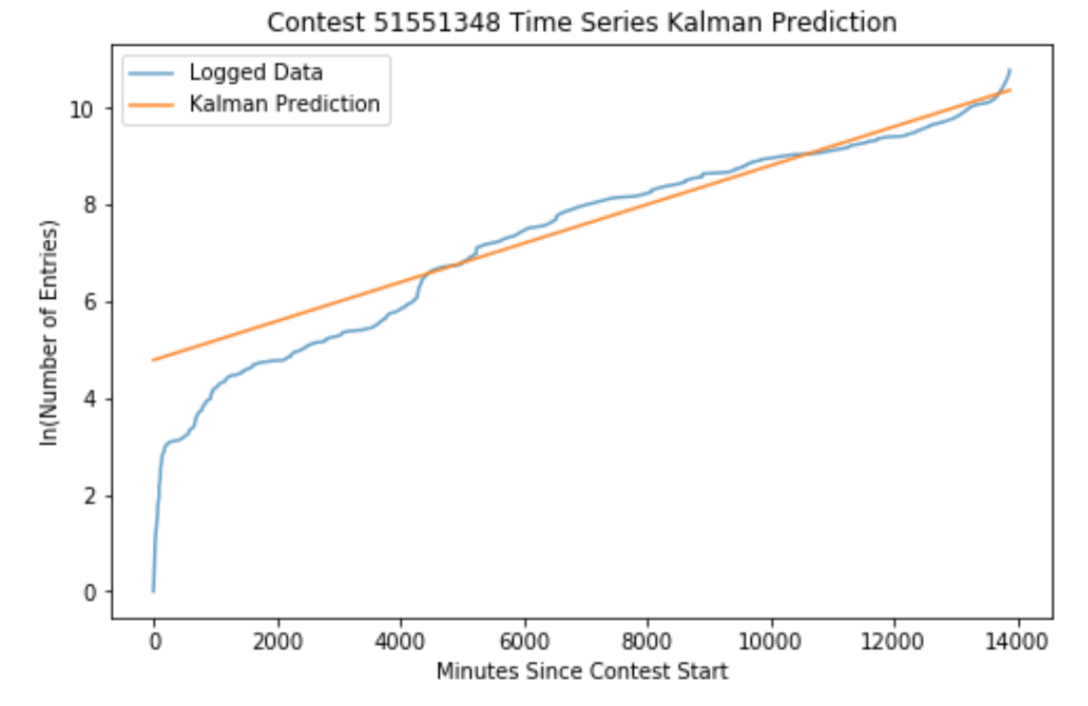
\includegraphics[width=8cm]{body/methodology/KF_Q0.png}
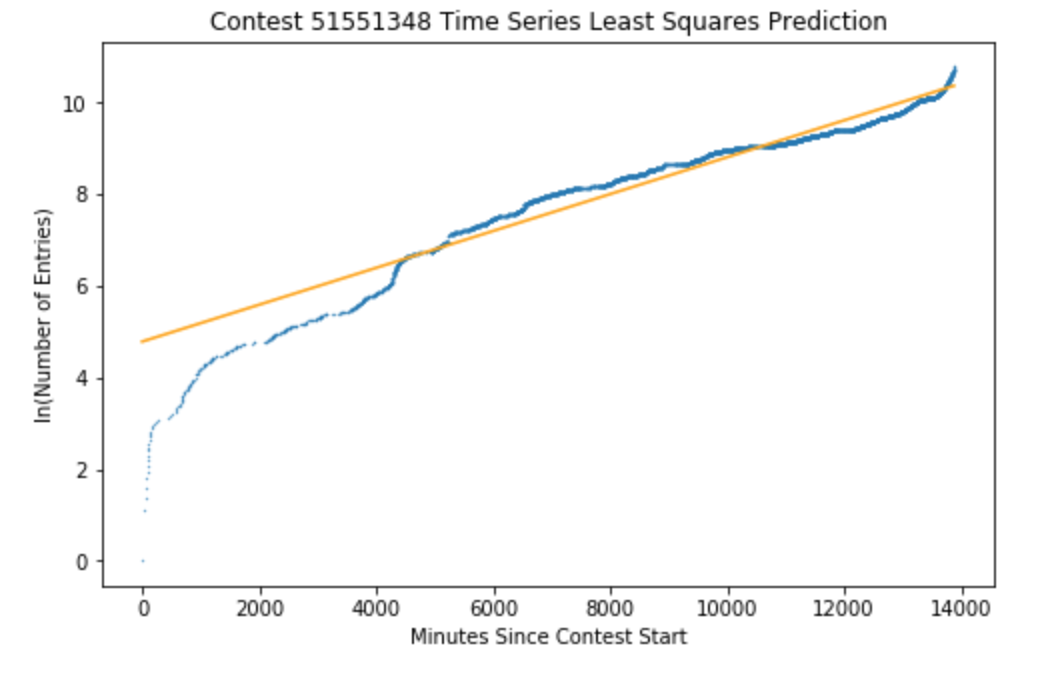
\includegraphics[width=8cm]{body/methodology/LS_pred.png}
\caption[Comparison of Least Squares and Kalman Filter Models]{The left image shows a linear regression performed on a real contest using the Kalman Filter with a $Q$ of all 0's. The right image shows a linear regression found using a weighted least squares fit on the same contest with $\lambda$ = 1. This is the case of no forgetting factor for both methods which can be seen to produce what looks like the same approximating function.}
\label{fig:kflsfit}
\end{figure}

Performing the fit by KF can be convenient for time series data as each iteration involves processing only one data point at a time. And while least squares is not very computationally intensive, it still requires redoing the entire dataset calculation when updating the parameter prediction.

\begin{figure}[h]
\centering
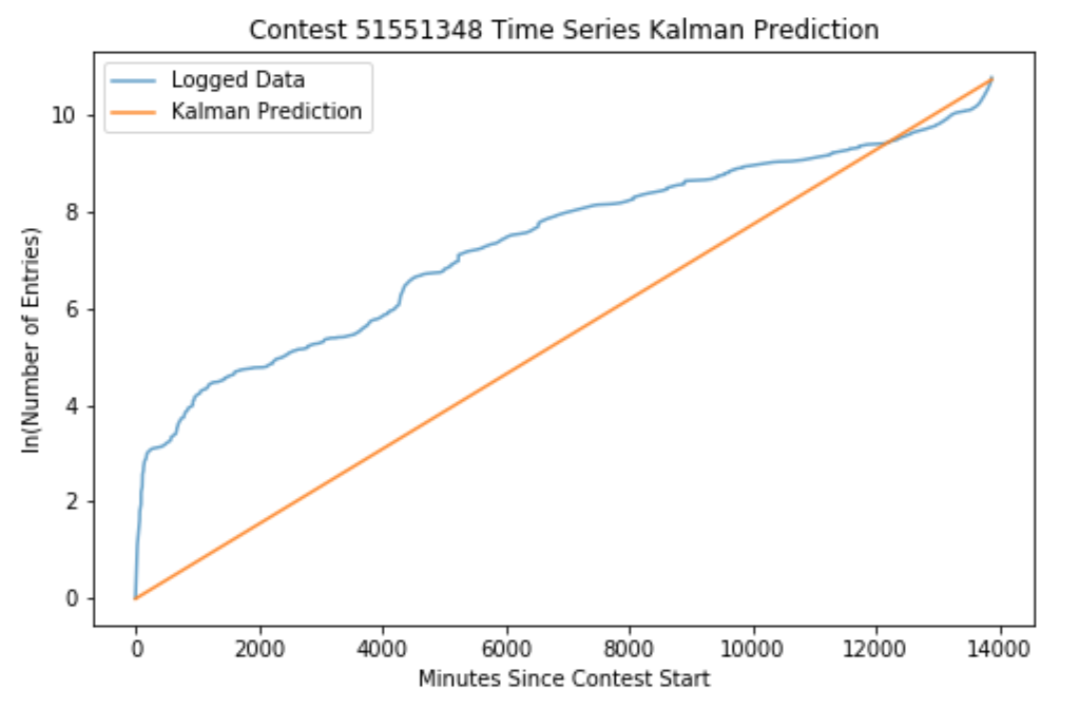
\includegraphics[width=10cm]{body/methodology/KF_Q3.png}
\caption[Modified Q Parameter Kalman Filter]{This is the same contest from Figure \ref{fig:kflsfit} except $Q_{\alpha}$ = 0.3. We can see that even a small change in the Q matrix produces a significantly different fitting function.}
\label{fig:q03fit}
\end{figure}

\subsection{Extended Kalman Filter}

While the KF is an excellent method for estimating model parameters, it is limited in the same way as LS in that it can only predict for linear models. This works for estimations on logged data, however, it'd be preferable to be able to directly estimate the parameters of the non-linear exponential function $\alpha e^{\beta t}$. To do this, we turn to the Extended Kalman Filter (EKF). The EKF works exactly the same as the normal KF except it can work with non-linear model functions. The only difference between the KF and EKF in this application is the values of $H_{k}$. For the EKF, $H_{k}$ takes the form

\begin{equation}
H_{k} = \begin{bmatrix}
           \frac{\partial M(t)}{\partial B_{1}} & \cdots & \frac{\partial M(t)}{\partial B_{i}}
         \end{bmatrix}
\end{equation}

where $B_{0} \cdots B_{i}$ are the values of the state space $\bm{\hat{x}}$ and $M(t)$ is the non-linear model function. In our case, we assume $M(t) = \alpha e^{\beta t}$, thus

\begin{equation}
H_{k} = \begin{bmatrix}
           e^{B_{1}t}&B_{1}B_{0}e^{B_{1}t}
         \end{bmatrix}
\end{equation}

Otherwise the calculations are exactly the same as for the ordinary KF. Figure \ref{fig:ekfexamp} shows some exponential model predictions using the EKF. $R = 30$ for both, but the left one has an all 0 $Q$ while the right has $Q_{\alpha}$ = $Q_{\beta} = 10$.

\begin{figure}[h]
\centering
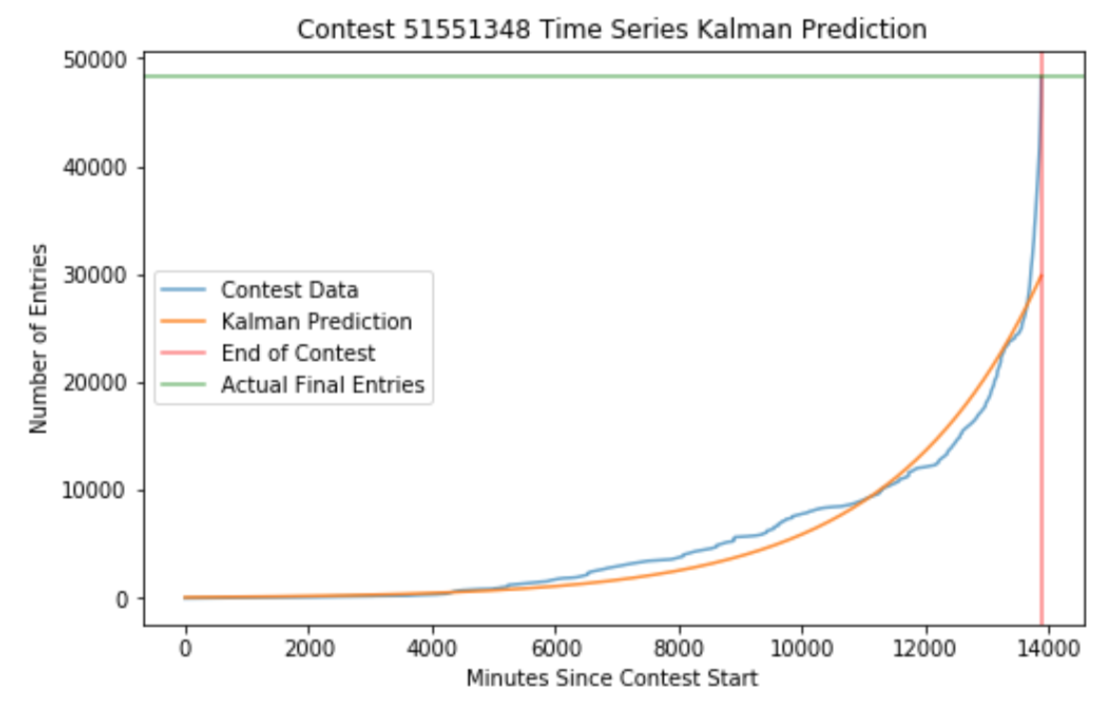
\includegraphics[width=8cm]{body/methodology/KF_True0.png}
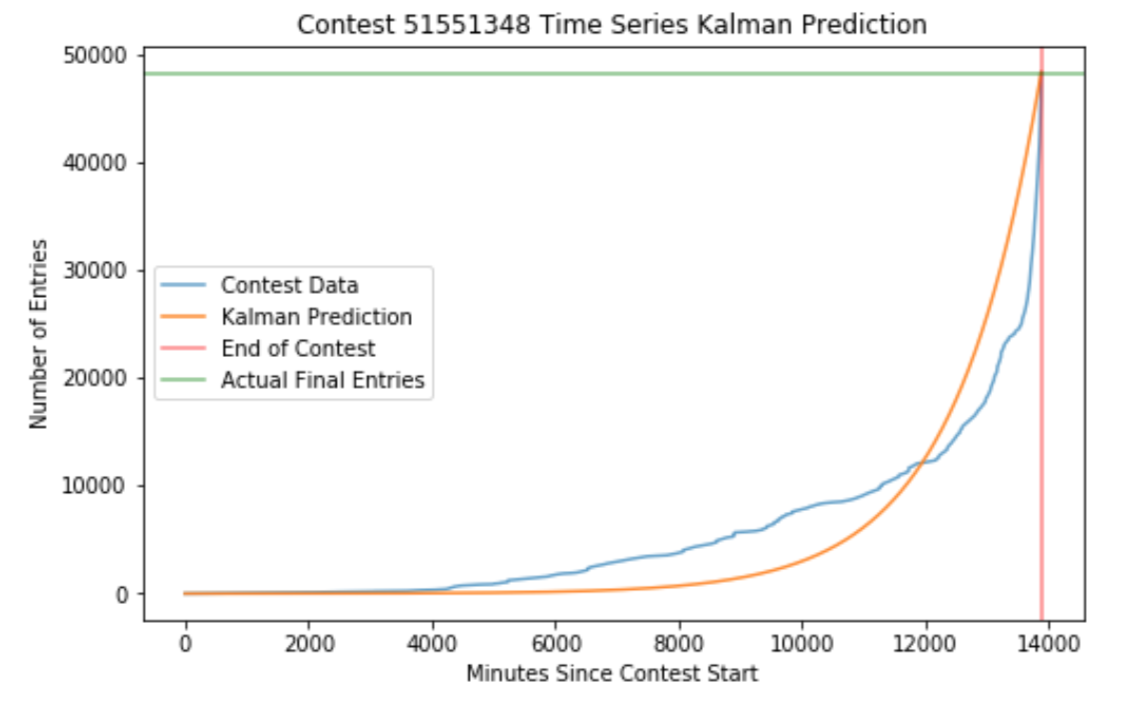
\includegraphics[width=8cm]{body/methodology/KF_True10.png}
\caption[Additional Varied Parameter Kalman Filters]{This is the same contest from Figure \ref{fig:kflsfit} with $R = 30$ for both. The left image is an exponential function found using a $Q$ of all 0's. The right image shows the exponential function found when $Q_{\alpha} = Q_{\beta} = 10$. Again, we can see how changing the $Q$ matrix produces a significantly different fitting function.}
\label{fig:ekfexamp}
\end{figure}